\RequirePackage{lineno}
\documentclass[12pt]{article}
\usepackage{graphicx}
\usepackage[caption=false]{subfig}
\usepackage{caption}
\usepackage{mathptmx}
\usepackage[T1]{fontenc}
\usepackage[absolute,overlay]{textpos}
\usepackage{fancybox}
\usepackage{multirow}
\usepackage[dvipsnames]{xcolor}
\usepackage{colortbl}
\usepackage{amsmath, amsthm, amssymb,amsfonts}
\usepackage{float}

%%% Code to enter C++ code
\usepackage{listings}
\lstset{language=C++,
        basicstyle=\ttfamily,
        keywordstyle=\color{blue}\ttfamily,
        stringstyle=\color{red}\ttfamily,
        commentstyle=\color{green}\ttfamily,
        morecomment=[l][\color{magenta}]{\#}
}

\usepackage{fullpage}
\usepackage{units}

\usepackage{hyperref}
\hypersetup{
    colorlinks,
    citecolor=blue,
    filecolor=black,
    linkcolor=black,
    urlcolor=black
}

\usepackage{xspace}

\author{Robert Kralik}
\title{\textbf{Data-based simulation of cosmic muons (not only) for calibration\\ \vspace*{5mm}
\Large{Technical Note}}}
\date{\today}

%\linenumbers % Include line numbers

\begin{document}
\maketitle
\begin{abstract}
In NOvA we use samples of stopping and through-going cosmic muons to calibrate our detectors. In order to verify that calibration procedure works for the simulated detectors as well as for the real detectors and to determine systematic uncertainties arising from calibration, we need to use a sample of simulated cosmic muons.

Originally we used (or still use) the CRY cosmic-ray generator to simulate a large Monte-Carlo (MC) sample and applied the same cosmic muon selections as for data. However the CRY simulation is extremely inefficient as only a very small fraction of the simulated cosmic-ray activity results in a selected calibration hits and most don't even hit the detector. This costs CPU, disk space, and file usage. The underlying momentum and angle distributions in CRY are also not well tuned to the NOvA sites, which may affect the calibration.

Data-based method of simulation eliminates the use of the CRY Monte Carlo generator. Instead, the detector activity artdaq-stage data files are passed through the beam removal filter, reconstruction chain, selection of good quality cosmic muons, charge assignment and smearing to be fed into the \texttt{"Text File Generator"}. 

This results in almost perfect efficiency as nearly every muon simulated makes it to the final MC calibration sample saving processing time, files, and storage. Additionally, the simulated muon distributions match the data by construction. Since the calibration chain is fairly time and CPU intensive itself, having fewer and smaller simulation files to calibrate also helps downstream of the file generation.
\end{abstract}

\newpage
\tableofcontents

\section{Introduction}
Data-based simulation of cosmic muons was first produced for the Test Beam detector calibration by Teresa Lackey in 2021. Teresa based the reconstruction and selection of data events on the \texttt{CerenkovSelection} module from light level tuning and wrote a simple python script for event smearing and muon charge assignment. This simulation was tested by Robert Kralik in 2021 and 2022 and showed significant discrepancies when compared to the period 2 Test Beam data.

The simulation was improved by Robert over 2022 and completed in 2023, with changed event selection and charge assignment and an added energy correction. It was used and tested in the calibration of the Test Beam detector in 2023.

This technical note explains the process to create simulation samples for calibration, with focus on the application in Test Beam. However, the process and the code were made general enough to be easily applicable for the Near and Far detectors, or to create a simulated sample of cosmic muons for non-calibration purposes.

\section{How does it work?}

All the code for creating data-based simulation of cosmic muons is located inside the novasoft \texttt{CosmicStudies} package.

The process to generate a new data-based simulation of cosmic muons starts with a sample of artdaq-stage data events containing information on Raw Digits hits. These are then filtered, reconstructed and selected to get the vertex positions and 4-momenta of cosmic muons. The \texttt{cosmicgenanajob} ART job produces a root file with a TTree containing all the necessary information, as described in section \ref{secCosmicGenAna}.

The reconstructed information for each event is then passed to a python script, which assignes a charge to each cosmic muon based on a statistical distribution. The python script also corrects the 4-momenta of the through-going muons to account for lost energy, smears the kinematic information to reduce bias on the input data and prints the \texttt{HEPEVT}-styled description of each event into a text file. This is decribed in section \ref{secPython}. 

(maybe cite the hepevt format MINOS wiki https://cdcvs.fnal.gov/redmine/projects/minos-sim/wiki/HEPEVT\_files

The text file is then passed to the \texttt{Text File Generator}, which uses the data information as seeds passed to the Geant4 detector simulation. By adding further reconstruction we create artdaq-stage simulation sample of cosmic muons. To create calibration samples of stopping and through-going cosmic muons we apply the same reconstruction and selection to the simulation sample as to any data sample. Details are described in section \ref{secGenerator}. 

Outline of all the necessary steps is in the box below and on the \href{https://cdcvs.fnal.gov/redmine/projects/novaart/wiki/DataDriven\_Cosmics}{DataDriven Cosmics Generation redmine wiki page}.

\vspace{5mm}
\fcolorbox{black}[HTML]{E9F0E9}{
\parbox{.9\textwidth}{
\begin{enumerate}
\item Run \texttt{cosmicgenanajob.fcl} on detector activity artdaq-stage files;
\item Hadd the outputs and run\\\texttt{GenerateHEPEVTFromROOT.py haddedOutput.root HEPEVTFileName.txt};
\item Split the resulting txt file into files each containing a subset of lines (events);
\item Generate FHiCL files each sourcing a different text file \\\texttt{CreateFclsForSimulation.sh TextFileGenjob\_template.fcl}\\ \hspace*{58mm}\texttt{inDir outDir};
\item Make a SAM definition from the FHiCL files with \texttt{sam\_add\_dataset};
\item Include all the text files into \texttt{TextFileGen.cfg} with \texttt{--inputfile};
\item Submit \texttt{TextFileGen.cfg};
\item Move the newly created simulation artdaq files to a persistent area, declare them to SAM and create a definition 
\item Generate the calibration files (pclist/pcliststop);
\item Move the results into a persistent location, declare to SAM and make definitions.
\end{enumerate}
}}

\subsection{Reconstruction and selection of cosmic muon events from data}\label{secCosmicGenAna}

The aim of the new simulation sample is to understand the differences between the real and the simulated detector. However, the original information coming into the simulation (the seed) is supposed to represent real data as close as possible, without introducing any biases due to reconstruction or selection. 

We need to study and understand the 

What is the aim of the simulation? To simulate a sample of comsic muons with symmetric kinematic distributions alike data. But also not biased by data, we want the Geant4 to do it's job and tell us what does the simulation think our detector does to the cosmic muons.

We want to select well reconstructed cosmic muons out of the detector activity artdaq-stage data sample and perform reconstruction to get the required kinematic information for each event. We also want the resulting simulation to be as small as possible without influencing the calibration. This means the selection should remove all the events that wouldn't make it to the final selection for calibration samples.

The first iteration also used Test Beam data from period 2 as an input, which include some FEB issues as well as underfilled cells 31 and 63 for all horizontal planes. This can negatively affect the resulting simulation in a non-trivial way. To avoid this for the second iteration, Robert used period 4 Test Beam data samples, which don't have the aforementioned effects. For details about the various conditions of the Test Beam detector and their effect on calibration and simulation see the Test Beam calibration technote (cite doc-db).

Both reconstruction and selection are done in a single job \textbf{\texttt{CosmicStudies/cosmicgenanajob.fcl}}.

\subsubsection{Remove Beam Spills}
The first step is to remove beam spill events using the \texttt{RemoveBeamSpills.fcl} job for the Near and Far Detectors, or \texttt{RemoveTBSpills.fcl} for the Test Beam detector, which should leave us with mostly cosmic events.

\subsubsection{Reconstruction}
The Text File Generator requires the vertex position and the initial 4-momentum for each event. For that we use:
\begin{enumerate}
\item \texttt{CalHit} to create Calibrated Cell Hits from Raw Digits,
\item \texttt{Slicer} to group hits into slices,
\item \texttt{Window CosmicTrack} - a tracking algorithm for cosmic particles,
\item \texttt{CosmicRayVertex} to identify vertices for cosmic particles,
\item \texttt{FuzzyKVertex} to cluster hits into prongs and
\item \texttt{BreakPointFitter (BPF)} to identify muons (or muon-like tracks) and get their initial 4-momenta by fitting to the FuzzyK prongs and CosmicRayVertex vertices.
\end{enumerate}

\subsubsection{Selection}
Following the reconstruction we select events based on their BreakPointFitter (BPF) tracks and momenta and on their slice properties and write them into a Root TTree. This step is done with the \texttt{CosmicStudies/CosmicGenAna} module. 

To select an event we require the following:
\begin{enumerate}
\item We are only using the muon assumption and successful fits from the BreakPointFitter;
\item There is a 3D reconstructed BPF track;
\item The distance of the start of each track from the Top/Front/Back/Sides of the detector is at most 50cm to only allow tracks starting outside of the detector. This cut has only negligible effect on the BPF tracks as can be seen on figure \ref{figCosZSelectionComparison};
\item Figure \ref{figCosZSelectionComparison} shows there are events peaked at track lengths $\sim 200$cm and $\sim 410$cm, which correspond to the total length of the detector and the half-length (length of one module). These are all strictly parallel to the beam direction (Cos$_Z\sim 1$) and are likely lefotver beam events. We can see that requiring the Z component of the unit angle (equal to Cos$_Z$) of the initial direction of the track to be less than 0.98 effectively removes these events without affecting the rest of the data;
\item The BPF track passes the PCHitsList cuts from \texttt{Calibration/PCHitsList} module. These cuts are applied to both data and simulation \textit{artdaq}-stage samples to create the \texttt{pclist} and \texttt{pcliststop} calibration samples. As this data-based simulation is intended mainly for calibration purposes, applying the PCHitsList cuts improves the selection quality without sacrificing any statistics as the same cuts will be applied further along the line. The cuts are:
\begin{itemize}
\item Tracks must have at least two X and two Y cells
\item The difference between the start and stop Z position of the track must be at least 70cm
\item The Z component of the initial direction vector of the track must be at least 0.2
\item At least 80\% of cells in slice must be reconstructed into the track in both X and Y views
\item At most 6 cells were hit per plane
\item Maximum difference between the first planes in X and Y is 3 (same for the last planes)
\item The difference between number of planes crossed in X and Y view must be at most 10\% of the total number of planes crossed
\item Remove tracks where a step between trajectory points is more than this value * the median step size
\end{itemize}

\begin{figure}
\subfloat{
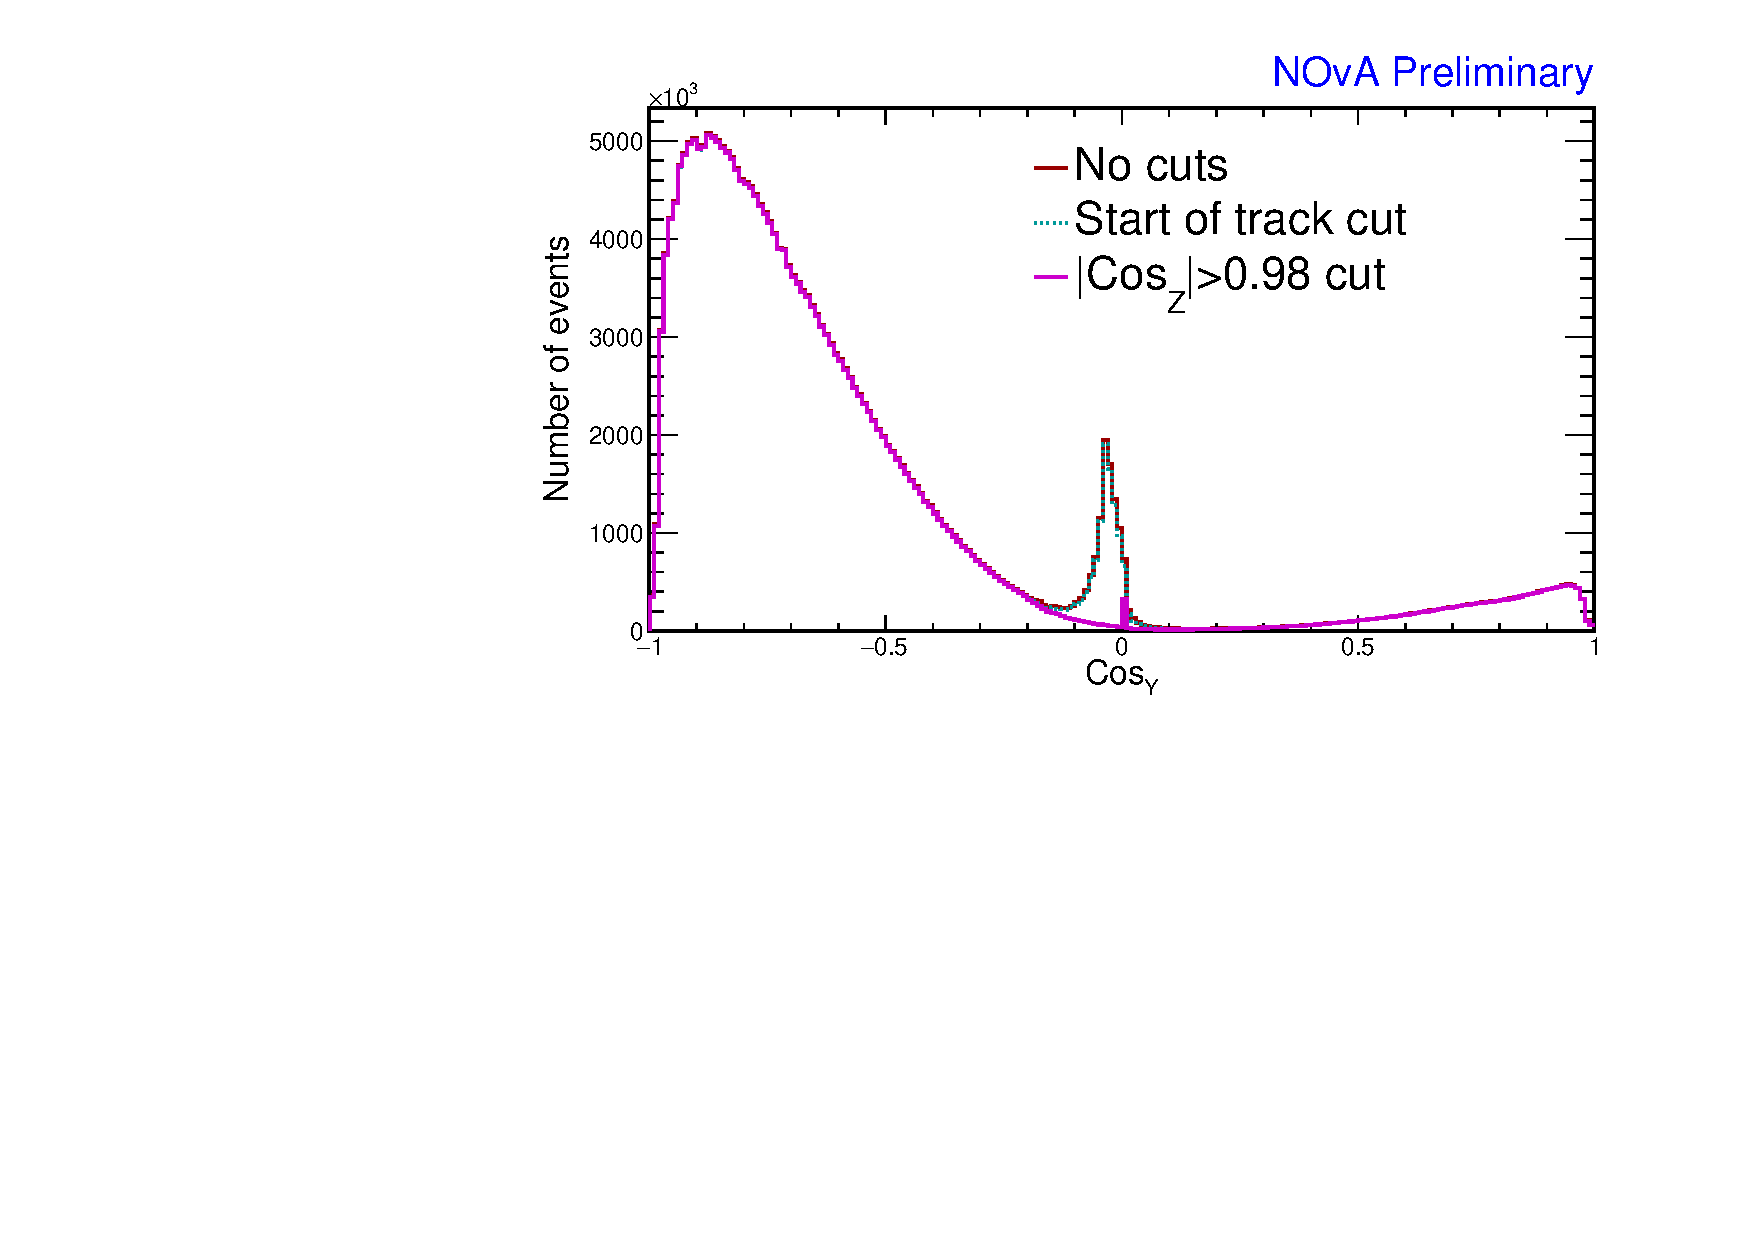
\includegraphics[clip, width=\textwidth]{SelectionComparisonCosZCut_CosY.pdf}
}

\subfloat{
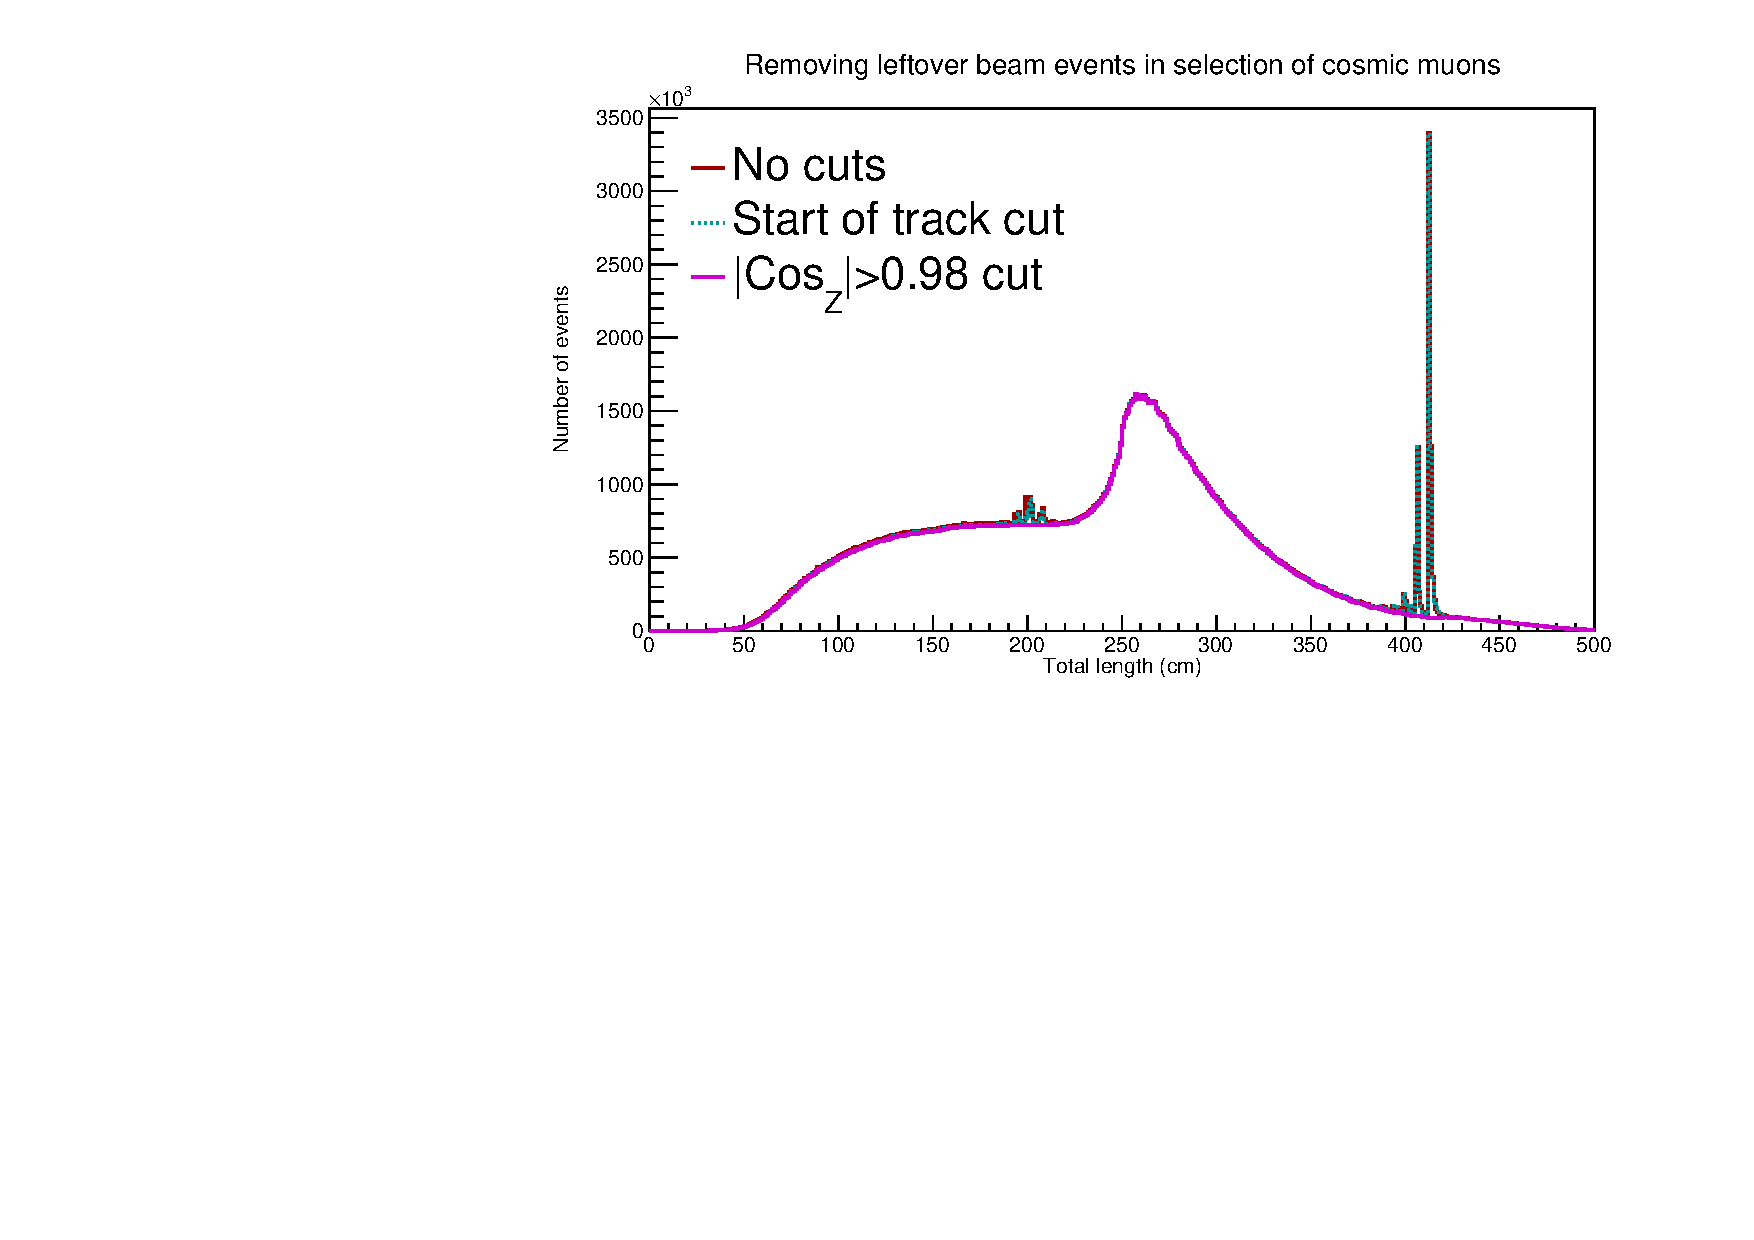
\includegraphics[clip, width=\textwidth]{SelectionComparisonCosZCut_TotLength.pdf}
}
\caption{Total track length distributions for different event selections. The original (blue) sample was used in the first iteration of the simulation for the test beam calibration by Teresa Lackey. The green line depicts the final selection of events. The peaks around 200cm and 410cm are beam events that made it past the RemoveTBSpills filter. The red line only includes the basic quality cuts from Break Point Fitter and requiring the existence of 3D tracks. The brown line shows distribution with all but the $Cos_Z$ cut applied.}
\label{figCosZSelectionComparison}
\end{figure}

There are two caveats to using these cuts decribed in sections \ref{secBPFvsWindowTrack} and \ref{secSelectionEfficiencyBias}. \textit{These cuts were not present for the first simulation iteration and were added by Robert Kralik for the second iteration};
\end{enumerate}

\begin{table}[]
\centering
\begin{tabular}{clcc}
& \centering{\textbf{Cut}} & \cellcolor[HTML]{3166FF}\textbf{Full selection} & \cellcolor[HTML]{32CB00}\textbf{Loose selection} \\ \hline
                                   & Muon assumption and 3D track from BPF         &                                             &                                          \\
                                   & Max. track start distance from edge                       & \multicolumn{2}{c}{50 cm}                                                                 \\
                                   & Max. $Cos_{Z}$                                            & \multicolumn{2}{c}{0.98}                                                               \\ \hline
                                   & Max. number of hits in X or Y                             & \multicolumn{2}{c}{\cellcolor[HTML]{FFFFFF}2}                                          \\
                                   & Min. difference between Stop$_{Z}$ and Start$_{Z}$        & \cellcolor[HTML]{3166FF}70 cm                 & \cellcolor[HTML]{32CB00}50 cm             \\
                                   & Min. $Cos_{Z}$ & \cellcolor[HTML]{3166FF}0.2                 & \cellcolor[HTML]{32CB00}0.15             \\
                                   & Min. frac. of slice hits in track in each view    & \multicolumn{2}{c}{0.8}                                                                \\
                                   & Max. number of cells per plane in each view               & \cellcolor[HTML]{3166FF}6                   & \cellcolor[HTML]{32CB00}15               \\
                                   & Max. difference in X-Y for first (last) plane     & \cellcolor[HTML]{3166FF}3                   & \cellcolor[HTML]{32CB00}5                \\
                                   & Max. plane asymmetry                                      & \cellcolor[HTML]{3166FF}0.1                 & \cellcolor[HTML]{32CB00}0.2              \\
                                   & Max. step size to median step size ratio                  & \cellcolor[HTML]{3166FF}3                   & \cellcolor[HTML]{32CB00}5                \\
                                   & \cellcolor[HTML]{C0C0C0}Max. vertex distance from edge    & \multicolumn{2}{c}{\cellcolor[HTML]{C0C0C0}10 cm}                                         \\
\parbox[t]{2mm}{\multirow{-10}{*}{\rotatebox[origin=c]{90}{PCHitsList cuts}}}& \cellcolor[HTML]{C0C0C0}Max. track end distance from edge & \multicolumn{2}{c}{\cellcolor[HTML]{C0C0C0}10 cm}
\end{tabular}
\caption{Table showing...}
\label{tabSelection}
\end{table}

During the selection process we also determine whether the muon is stopping inside the detector, or passing through, based on the end position of its reconstructed track. This helps us to correct the energy of the through-going muons to account for "lost energy" as described in section \ref{secPython}. \textit{For Test Beam we say it is a stopping muon if its track ends at least 20cm (for far and near detector this is 50cm) from any edge of the detector. This value was chosen by Kevin Mulder \cite{NOVA-doc-39244-v1} as 50cm removed too many cosmic events from the Test Beam detector.} 

During the first iteration of the simulation, Teresa applied a cut on the total track length to be at least 300cm. This was motivated by the Cerenkov selection for the light level tuning, but it was the main cause of the data-simulation discrepancy for the calibration samples. Robert Kralik removed this cut and to assure that the quality of selected events remains good, applied the cuts from PCHitsList and a cut on the $Cos_Z$ to remove remaining beam events. Figure \ref{figTotLengthCutComparison} shows the stark difference between this "Original selection (2021)" and the final selection used for the simulation. 

\begin{figure}
\subfloat{
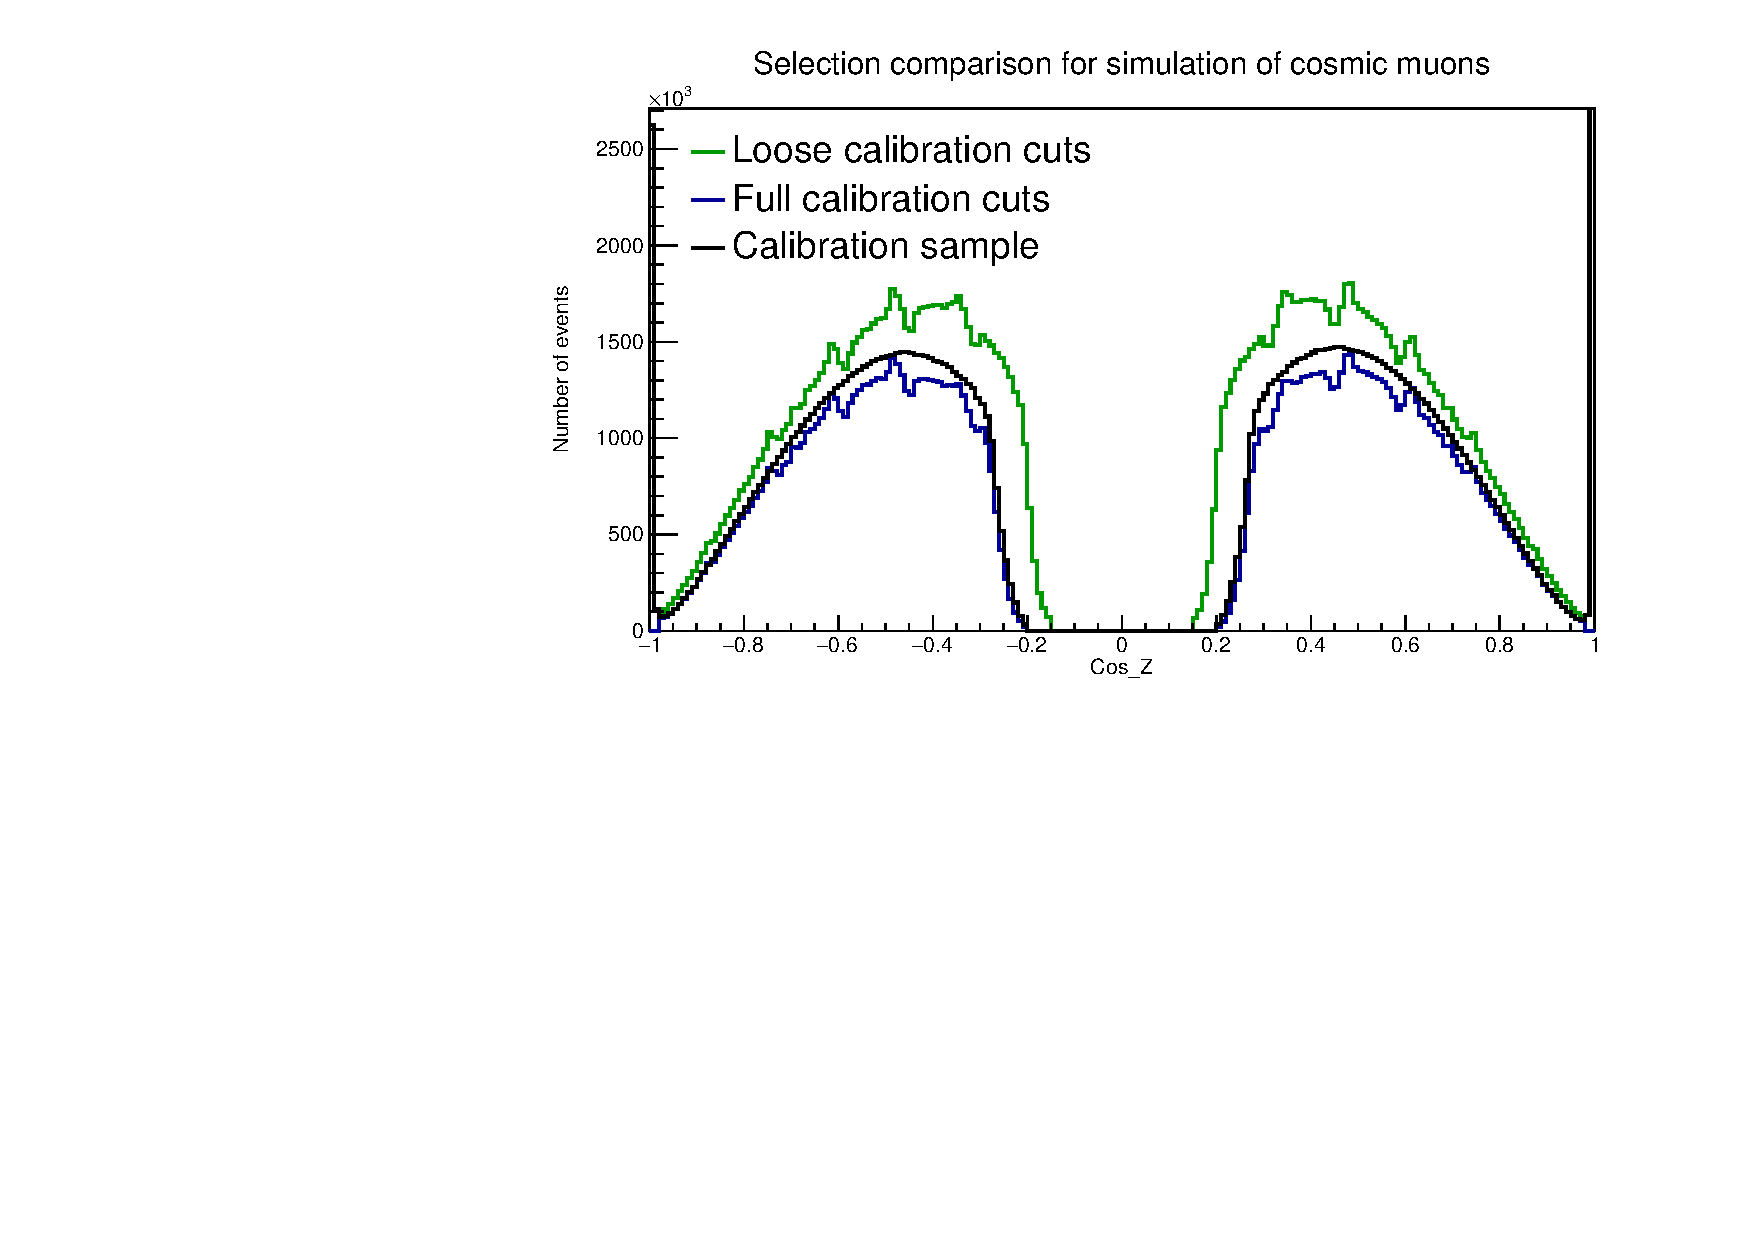
\includegraphics[clip, width=\textwidth]{SelectionComparisonPCHitsListCut_CosZ.pdf}
}

\subfloat{
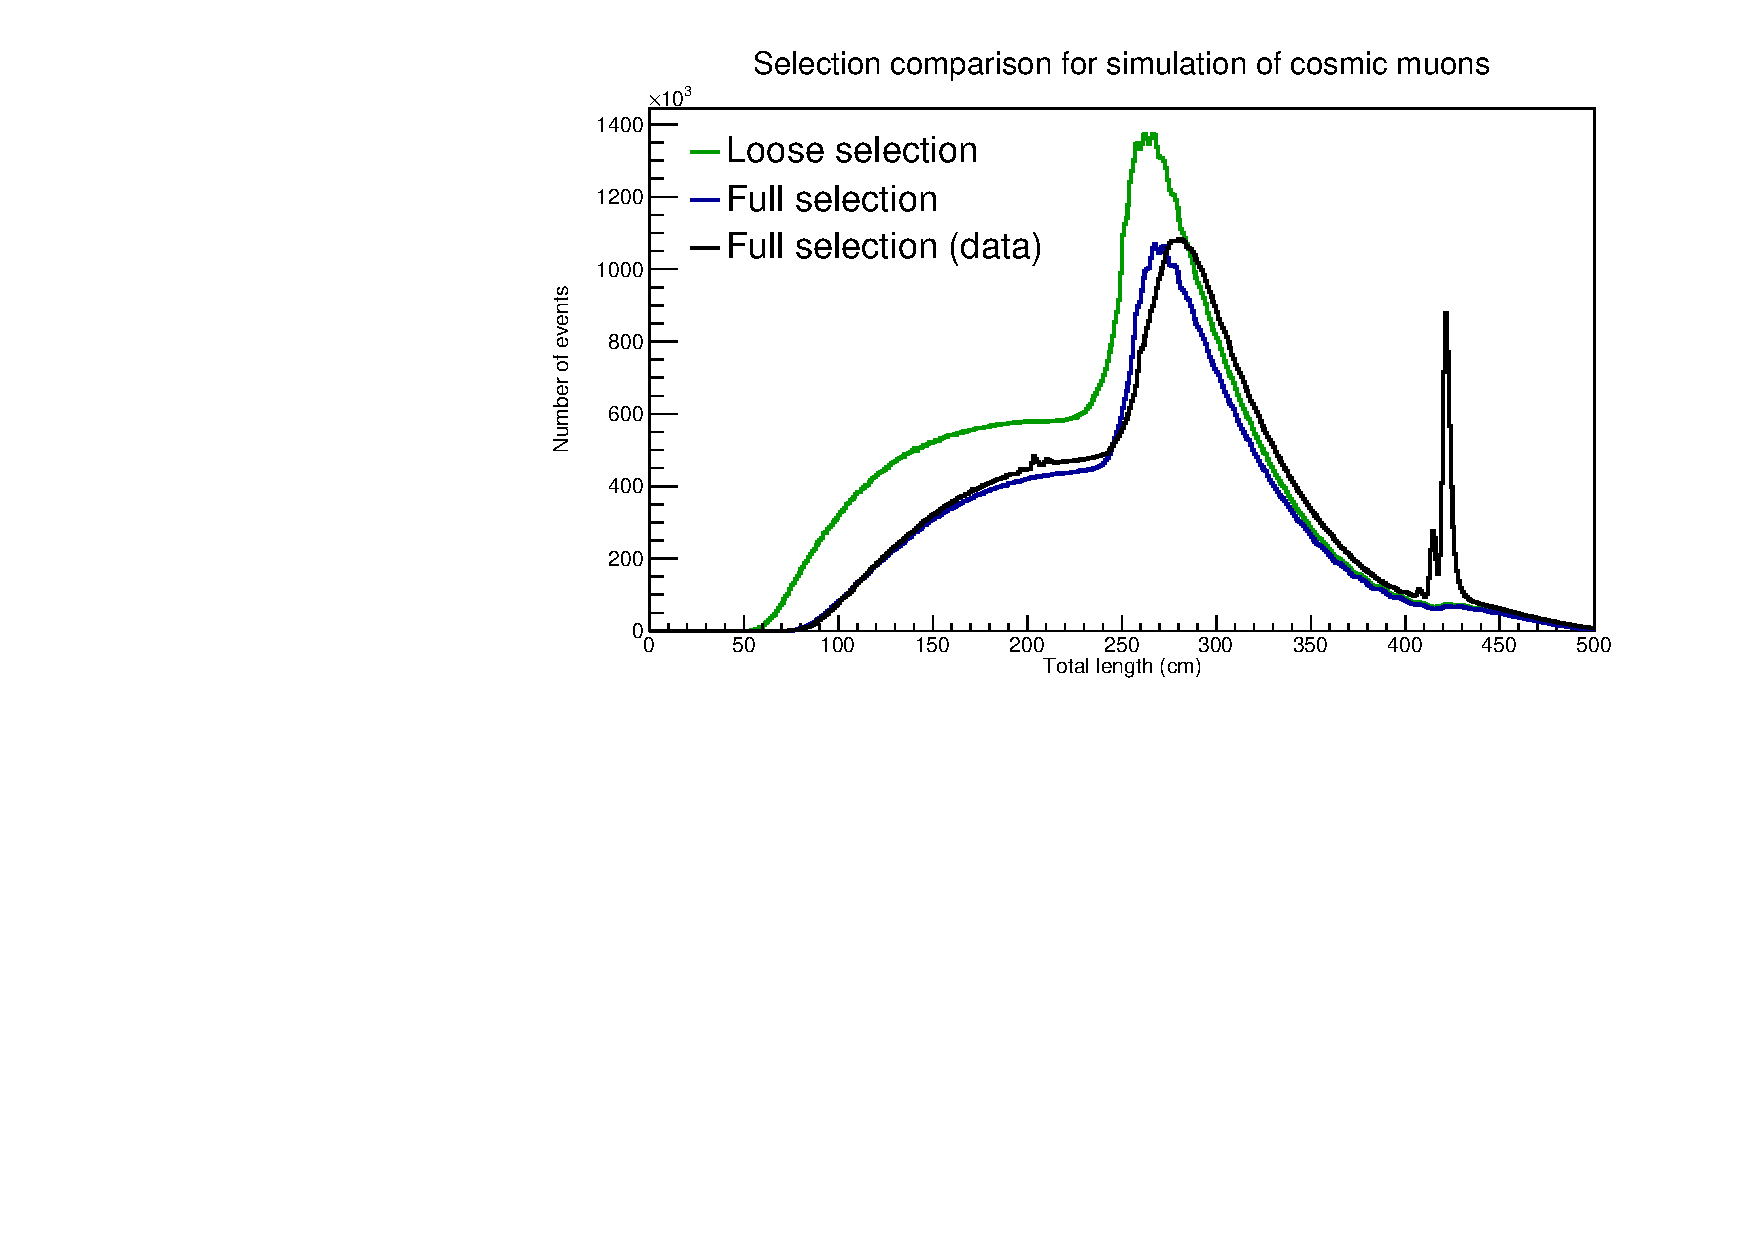
\includegraphics[clip, width=\textwidth]{SelectionComparisonPCHitsListCut_TotLength.pdf}
}
\caption{Total track length distributions for different event selections. The original (blue) sample was used in the first iteration of the simulation for the test beam calibration by Teresa Lackey. The green line depicts the final selection of events. The peaks around 200cm and 410cm are beam events that made it past the RemoveTBSpills filter. The red line only includes the basic quality cuts from Break Point Fitter and requiring the existence of 3D tracks. The brown line shows distribution with all but the $Cos_Z$ cut applied.}
\label{figTotLengthCutComparison}
\end{figure}

The original PCHitsList cuts are:
\begin{itemize}
\item Tracks must have at least two X and two Y cells
\item The difference between the start and stop Z position of the track must be at least 70cm
\item The Z component of the initial direction vector of the track must be at least 0.2
\item At least 80\% of cells in slice must be reconstructed into the track in both X and Y views
\item At most 6 cells were hit per plane
\item Maximum difference between the first planes in X and Y is 3 (same for the last planes)
\item The difference between number of planes crossed in X and Y view must be at most 10\% of the total number of planes crossed
\item Remove tracks where a step between trajectory points is more than this value * the median step size
\end{itemize}

\subsubsection*{BPF track VS window\_cosmictrack difference and effect}\label{secBPFvsWindowTrack}
%However, since the CosmicGenAna class uses the BPF tracks and the PCHitsList class uses the Window\_cosmictrack tracks for selection, there may be some biases introduced by using all the PCHitsList cuts without adjustments.

The PCHitsList cuts used to create the calibration samples use tracks from the \texttt{Window\_cosmictrack} algorithm, since we do not need the 4-momentum information. However we need to use the Break Point Fitter tracks for our selection. As we can see on figure \ref{figTrackAndCutComparison}, there is a non-negligible difference between the distributions of the two tracking algorithms. 

Show some plots and explain why is this a problem, but also if using the original PCHitsList cuts introduces bias for the simulation samples. Maybe point to some of my talks for reference (?).

\begin{figure}
\centering
\subfloat{
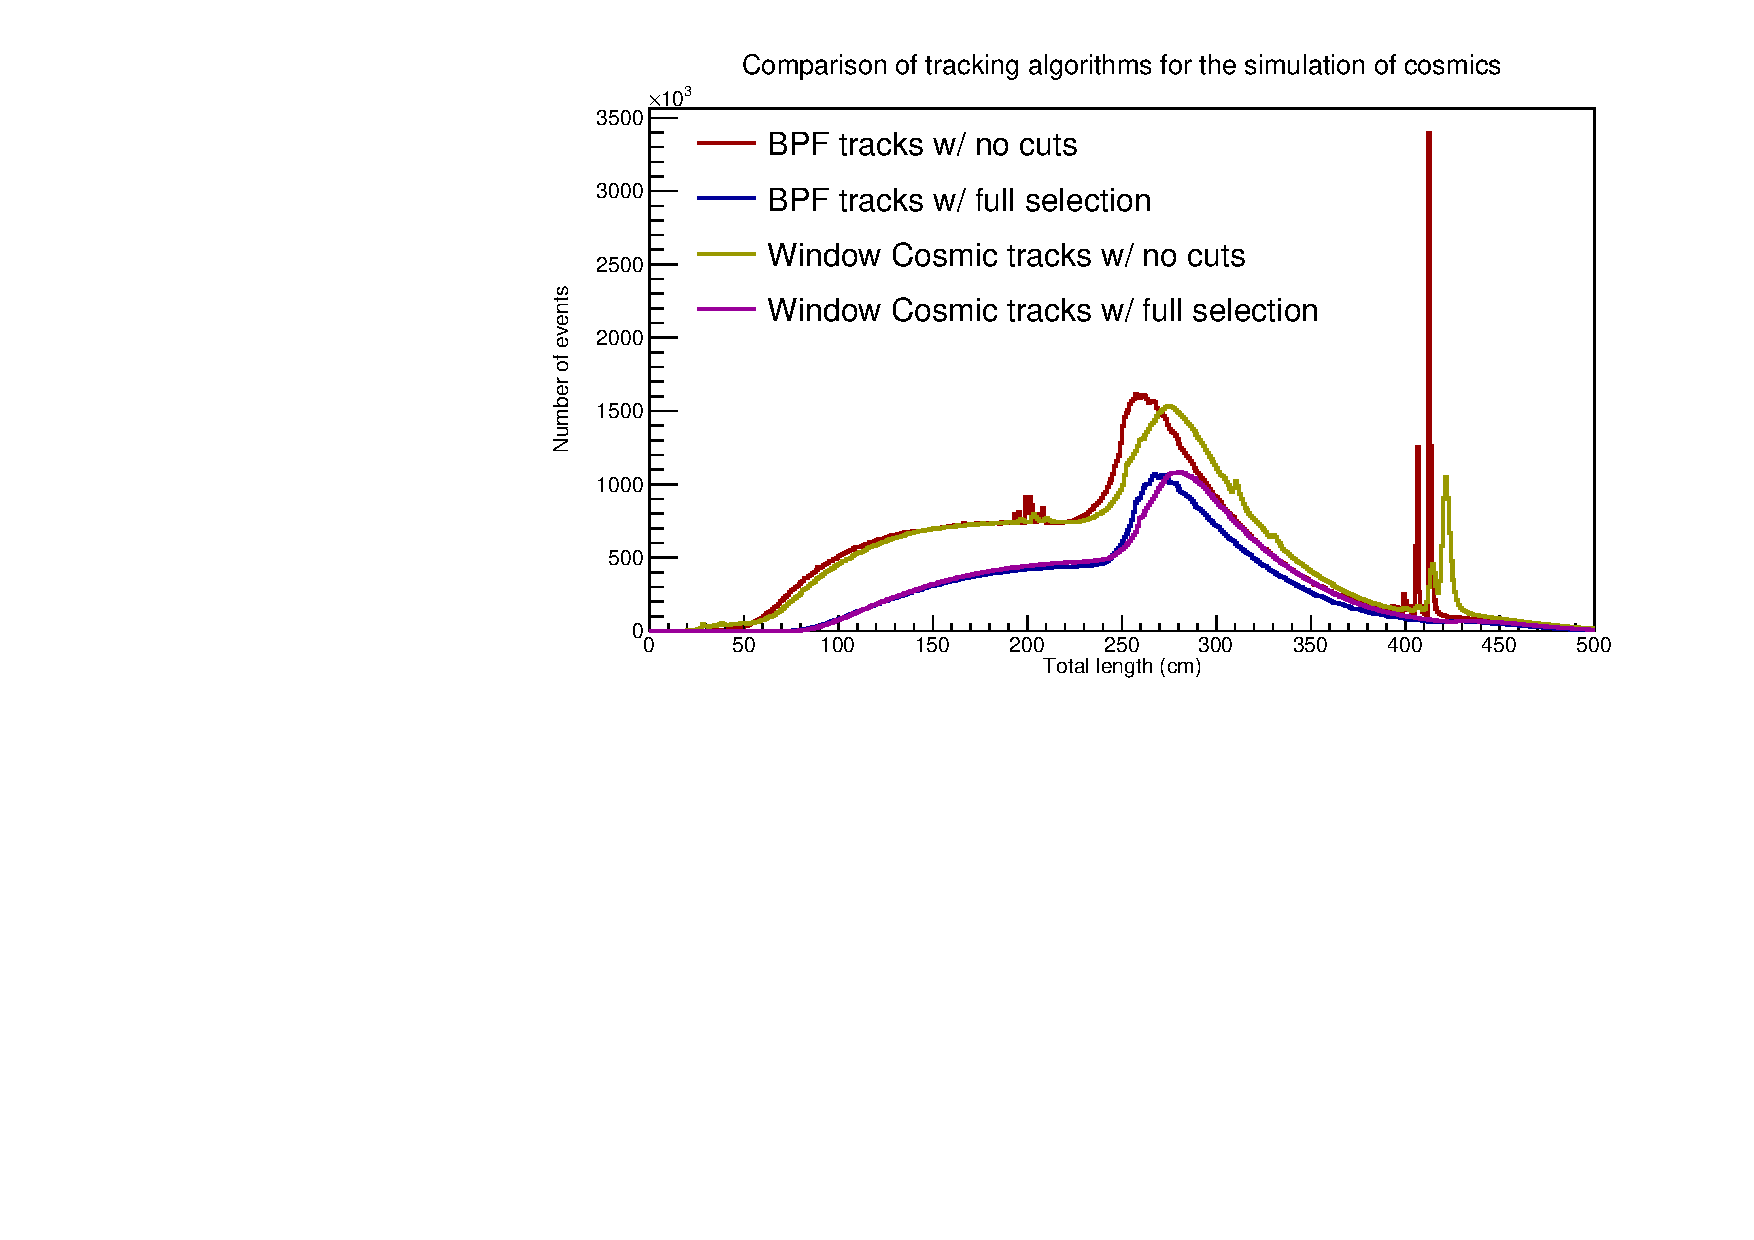
\includegraphics[clip, width=\textwidth]{TrackAlgComparison_TotLength.pdf}
}

\subfloat{
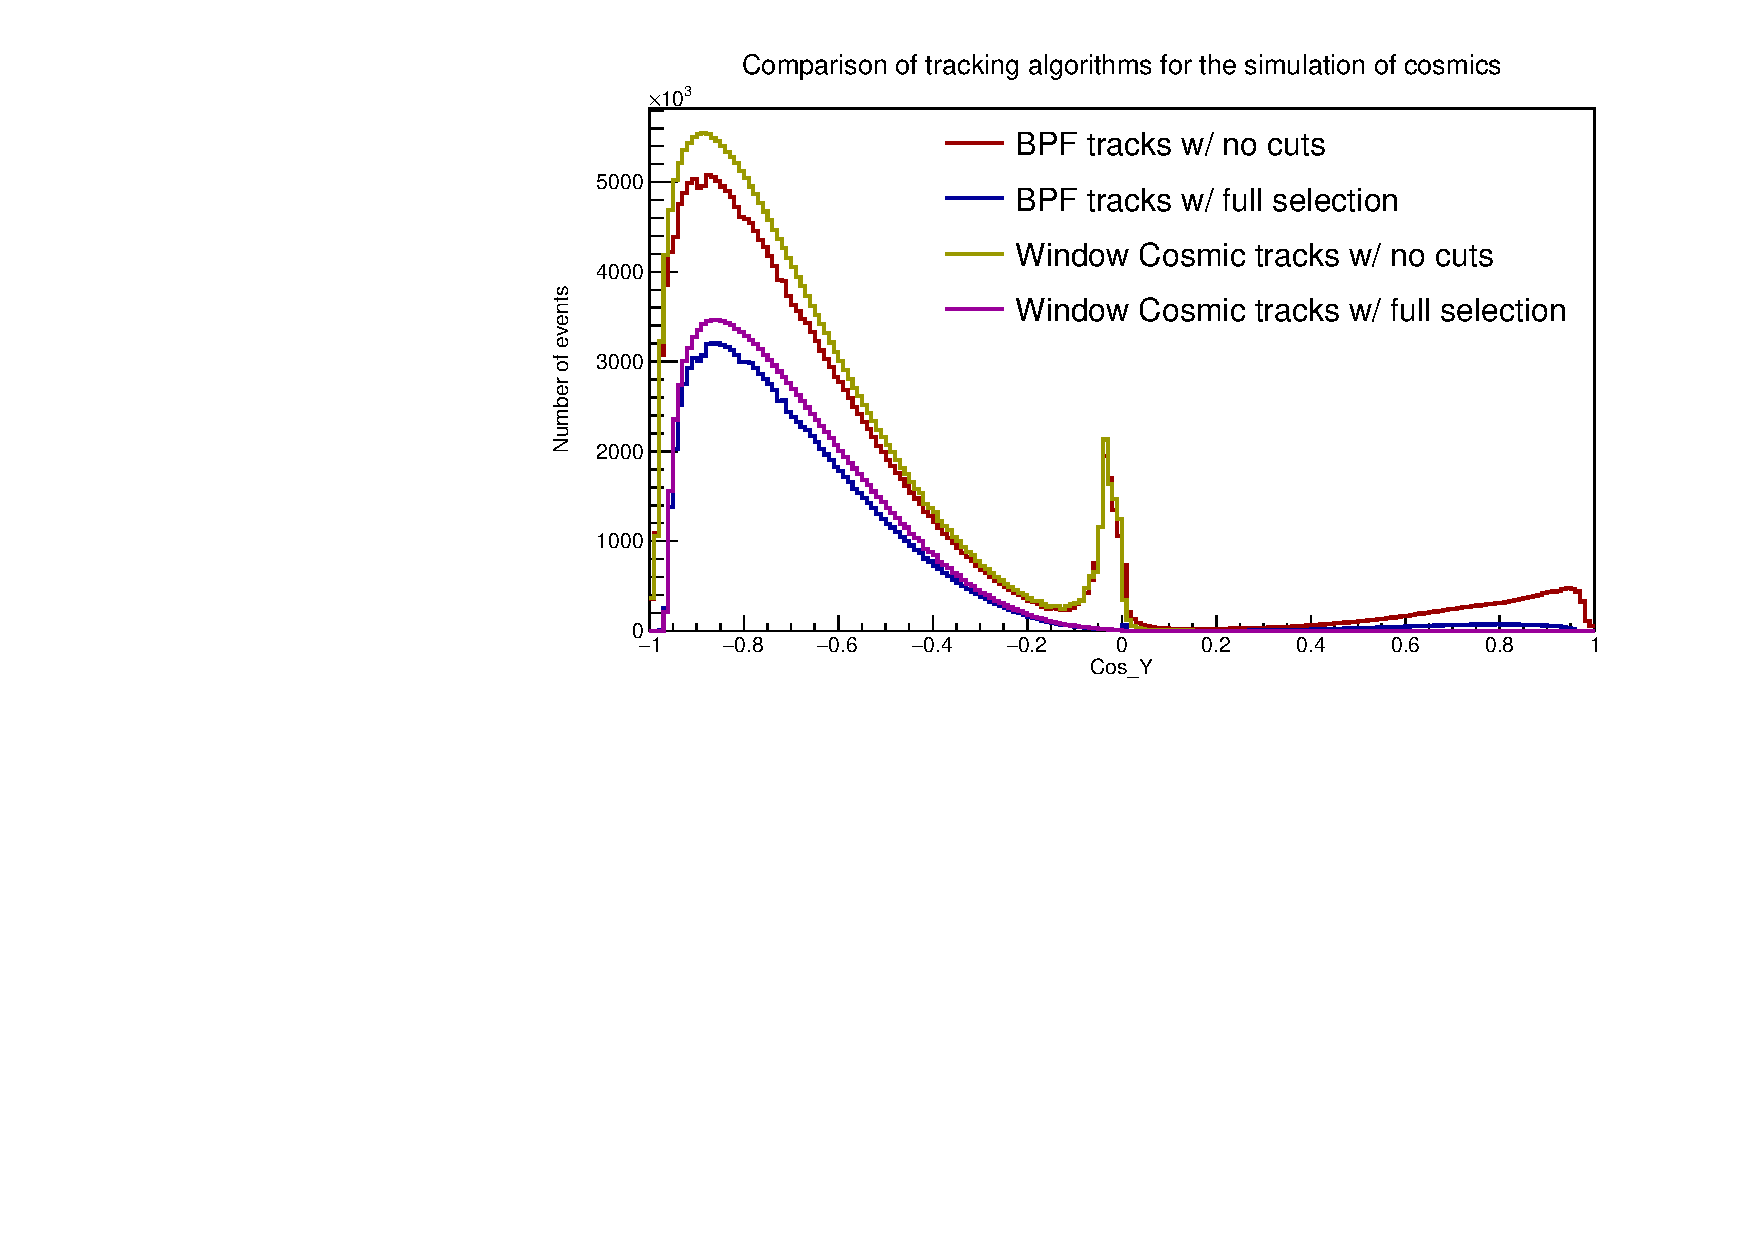
\includegraphics[clip, width=\textwidth]{TrackAlgComparison_CosY.pdf}
}

\caption{Distributions of the total track length (top) and the angle from the Y axis for different track reconstruction algorithms and selections.}
\label{figTrackAndCutComparison}
\end{figure}

\subsubsection*{Selection efficiency bias}\label{secSelectionEfficiencyBias}

The reconstruction algorithms we use are never perfect which can result is some events theat were supposed to be selected not passing our selection. This can create and undesired bias as the distribution of events passed to the simulation may not correspond to the true distribution of data.

We can aleviate this bias by using a looser selection than desired which should leave a room for events with slightly incorrect reconstruction.

To validate whether our solution is working we use the result of the simulation as the "fake data" input for a second iteration of simulation and repeat every same in the exact same way. If the first and the second iteration of the simulation have a shift between each other, it means there's a selection efficiency bias.

\subsection{Energy correction, charge assignment and smearing}\label{secPython}
During one of the detector systematics planning sessions in Summer 2021, Mark Messier and Teresa Lackey presented an overview and a strategy for data-based simulation of cosmic muons for calibration (see \cite{NOVA-doc-51327-v3}). Mark and Teresa outlined possible improvements to the energy estimation of the through-going muons, muon charge assignment based on energy distributions and the plan for application to the NOvA standard detectors (ND/FD).

Once we have the TTree we run a python script \texttt{generate\_hepevt\_cosmic.py}. This script uses the \texttt{uproot} library to load the TTree ntuples into a dictionary of numpy arrays. Uproot might not be installed on the machine you're using. You can run \texttt{pip install --user uproot} to install it.

To run the python script do:
\begin{lstlisting}[frame=single,language=bash]
python generate_hepevt_cosmic.py inFile.root outFile.txt\
                                 --niter NIterations
\end{lstlisting}

\subsubsection{Energy correction}
Muons that do not stop inside the detector carry away the energy not deposited in the detector and their true initial energy is therefore larger than the reconstructed energy $E_R$ we get from the Break Point Fitter. In general, the energy spectrum of cosmic muons can be approximately described by a power law $E^{-\alpha}$, with $\alpha\approx2.7$ \cite{NOVA-doc-51327-v3}. The expectation value for the "true" energy of the through-going muons can be calculated as
\begin{equation}
\left\langle E\right\rangle =\frac{\int^{E_C}_{E_R} E\cdot E^{-\alpha}}{\int^{E_C}_{E_R} E^{-\alpha}}=\left(\frac{\alpha -1}{\alpha -2}\right)\left(\frac{E_C^{2-\alpha}-E_R^{2-\alpha}}{E_C^{1-\alpha}-E_R^{1-\alpha}}\right)
\end{equation}
where $E_C$ is the critical energy chosen to be 300GeV, as we do not expect muons with higher energies to be selected due to large showers along their paths. Plot \ref{figEnergyScaling} shows that the choice of the critical energy does not significantly change the correction of the true energy.

Need more reliable source of the equation!
Page 9 of the PDG, equation (30.4):
https://pdg.lbl.gov/2022/reviews/rpp2022-rev-cosmic-rays.pdf

\begin{figure}[hbtp]
\centering
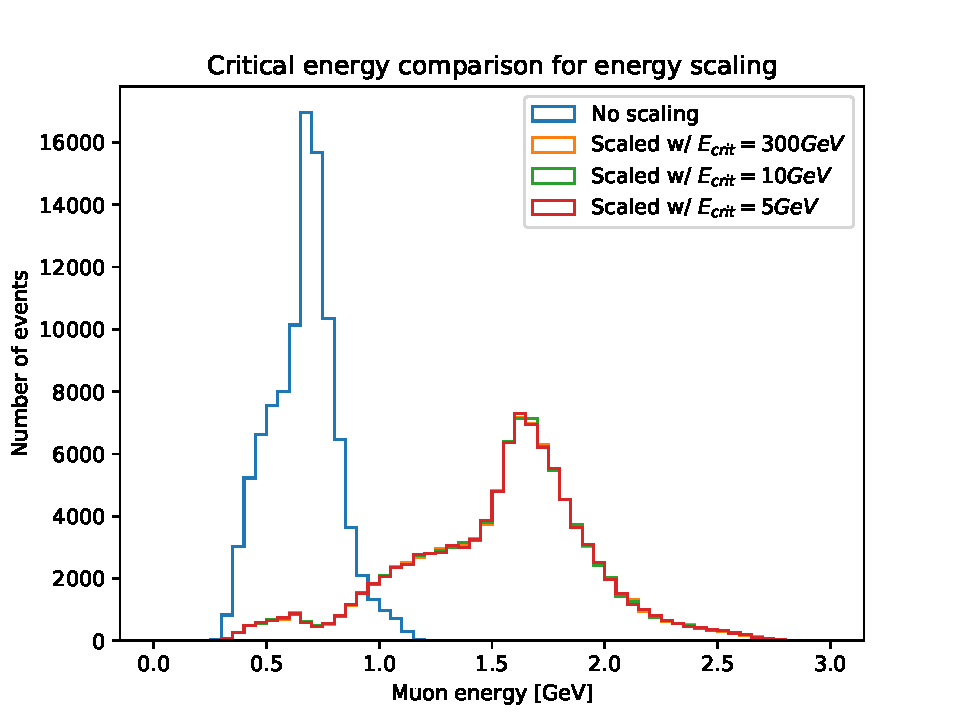
\includegraphics[width=0.8\textwidth]{ECritComparison.pdf}
\caption{The effect of energy correction for through-going muons with various critical energies. No significant difference can be seen when using different critical energies.}
\label{figEnergyScaling}
\end{figure}

\subsubsection{Smearing}
Smear the events to avoid any bias from the data. Smearing is done by randomly changing the total momentum within 2\%, azimuthal angle uniformly, polar angle within 4mrad and the X/Y and Z vertex positions within the width or depth of the cell respectively.

\subsubsection{Charge assignment}
Text File Generator requires the charge of each muon event. Since we reconstruct muons and antimuons in the same way, we have to assign the charge based on external measurments.

Figure out where are the plots and the equation Mark/Teresa quoted from (somewhere in PDG). Describe the basis of the measurement.
Here(p10): https://pdg.lbl.gov/2022/reviews/rpp2022-rev-cosmic-rays.pdf
But the equation must be from one of the sources listed.

\begin{equation}
P_+ \simeq 0.539 + \frac{x}{34.5}-\left(\frac{x}{9.48}\right)^2 + \left(\frac{x}{8.27}\right)^3
\end{equation}

\subsubsection{Number of events to simulate}
The python script also contains options to multiply (\texttt{niter}) or skip (\texttt{stride}) events to adjust the statistics. We do not want to simulate too many events unnecessarily, as this would require larger memory and computational resources during calibration and therefore diminish one of the major benefits of data-based simulation.

We also need enough events to be able to comfortably calibrate the entire simulated detector. This means that in each cell, view and every one of the 12 fiber brightness bins we need enough through-going muons for the attenuation fit to have $\chi^2<0.2$.

From observation, the good number of \textbf{tricell hits} for each cell X view X brightness bin is $\sim$50,000. This is the same for Test Beam, Near and Far detectors, since the binning in the position within cell (w) is the same for all detectors. We have to account for 
The vertical cells have ~5x fewer hits than horizontal cell, so we need to multiply this by Y view + X view (=5x Y view) = 6x Y view.
Multiply this by number of fiber brighness bins, which is the same for all detectors, 12.
Multiply this by number of cells. This is 390 for FD, 100 for ND and 64 for TB.
For TB we get 200*100*6*12*64 = 92,160,000. That's the minimal number of tricell hits we need in total.

Since we are simulating events not hits and each event can have a vastly different number of successful tricell hits, we need to estimate. There's 7.5 more cell hits than tricell hits (13\%). Event has on average 5 tricell hits (37 cell hits).
So for Test Beam we need ~ 18,432,000 events.
Plus only about 90\% of simulated events end up in the detector and pass the PCHitsList cuts.
So for Test Beam we need to simulate at least 20,480,000. From period 4 we get 159,153,260 events with loose selection and 132,420,230 events with full selection. So this should be plenty for a successful calibration, maybe event too large.

All detectors have the same binning in w for relative calibration.
FD: maxPlane=900, maxCell=390. ND: maxPlane=220, maxCell=100. TB: maxPlane=63, maxCell=64

\subsubsection{Print the outputs}
Write the pdg code, 4-momentum components and vertex positions into a hepevt-format text file which will then be fed to the TextFileGenerator.

\subsection{Submitting the simulation jobs}\label{secGenerator}
\begin{enumerate}
\item The output of \texttt{generate\_hepevt\_cosmic.py} script is a single large \texttt{.txt} file (let's call it \\ \texttt{TextGen\_inFile.txt}. To run it on the grid, split it into multiple subfiles, each will be sourced by a separate \texttt{FHiCL} file. Don't forget that each event is written on 2 lines in the \texttt{txt} file, so split it into an even number of lines. From experience, 125,000 events (250,000 lines) are optimal, where each job runs for only a few hours. 250,000 events could be considered if the number of created subfiles would be >1000.
\begin{lstlisting}[frame=single,language=bash]
split -d -l 250000 --additional-suffix=.txt\
TextGen_inFile.txt /path/to/new/files/TextGen_inFile_
\end{lstlisting}

\item Then create the same amount of FHiCL files, each sourcing a different text file. There is a template called \texttt{TextFileGenTBjob\_template.fcl}. Take a look at it and check (not only):
\begin{itemize}
\item maxEvents
\item firstRun, firstSubRun
\item physics.producers.photrans.nd/fd/tb.BrightnessFile (which brightness file is used for the simulation)
\end{itemize}

The brightness file describes the relative differences in energy response across the different cells and planes. These differences mainly arise from the variability of each fiber's brightness, and specifically for test beam also from the different scintillators used. Since we want the simulated detectors to be functional copies of the ideal versions of the real detectors, it is important to provide a correct brightness file without any defects. More information about the brightness files and how to create them can be found on the \href{https://cdcvs.fnal.gov/redmine/projects/novaart/wiki/Test\_Beam\_Calibration\_Instructions}{Test Beam calibration redmine wiki page}.

In the first iteration of the data-based simulation, Teresa used a test beam brightness file created from period 2 data, which contains faulty FEBs and underfilled cells, resulting in a simulation also containing these defects. In the second iteration Robert created a new brightness file from period 4 test beam data, which are free from any irregularities and supplied that to the simulation

\begin{lstlisting}[frame=single,language=bash]
bash CreateFclsForSimulation.sh
     TextFileGenjob_template.fcl
     /path/to/TextGen_infiles_directory/
     /path/to/output/TextGen_fcl_directory
\end{lstlisting}

\item Then create a SamWeb definition out of these FHiCL files
\begin{lstlisting}[frame=single,language=bash]
sam_add_dataset -n username_CosmicGen_description
                -t username_date
                -d /path/to/FHiCL/directory
\end{lstlisting}
You can also use the option \texttt{--no-rename} if you've named your FHiCL files uniquely enough.

\item Adjust the configuration script accordingly (\texttt{njobs}, \texttt{defname} for your fcls, \texttt{dest},...) and include all the text files with:
\begin{lstlisting}[frame=single,language=bash]
for file in $(ls -1 /path/to/TextGen_inputfiles/*); do
echo --inputfile $file >> TextFileGen.cfg; done
\end{lstlisting}
If you need to remove the previously included text files, you can do
\begin{lstlisting}[frame=single,language=bash]
sed -i '/^--inputfile/d' TextFileGen.cfg
\end{lstlisting}

\item Submit. First with the \texttt{--test\_submission} flag and if everything looks all right, comment it out.
\begin{lstlisting}[frame=single,language=bash]
submit_nova_art -f TextFileGen.cfg
\end{lstlisting}

\item This results in artdaq-stage simulation files. Move them to a suitable area for long storage (for example persistent, ask production) and investigate them. You can re-use the CosmicGenAna module from section \ref{secCosmicGenAna}.

\item To create the calibration samples you can ask prodction to create them for you or to point you to a corresponding job to use. For Test Beam you can use \href{https://github.com/novaexperiment/novaprod/blob/main/novaproduction/fcl/testbeam/prod\_tb\_ddactivity1\_pclist\_mc\_job.fcl}{this} script
\begin{lstlisting}[frame=single,language=bash]
novaprod/novaproduction/fcl/testbeam/
prod_tb_ddactivity1_pclist_mc_job.fcl
\end{lstlisting}
This creates the simulation calibration samples. You should move them a suitable area (like persistent) and create new definitions from them. You can again ask production for help.
\end{enumerate}

\section{Validation}
Show plots and decribe data-MC comparison and gen3 to gen3.5 and gen3.7 comparisons. Maybe also refer to the TB calibration technote to see how was this simulation employed.

\section{Conclusions}
Do we need this?

\bibliographystyle{unsrturl}
\bibliography{DataBasedCosmicsTechNoteLiterature}
\end{document}